\documentclass[12 pt, a4paper]{report}
%\documentclass[runningheads]{llncs}
\usepackage[T1]{fontenc}
\usepackage{mathptmx}
\usepackage{amsmath,amssymb,amsfonts, amsthm}

\theoremstyle{definition}
\newtheorem{definition}{Definition}[section]

\usepackage{setspace}
%\usepackage[top=1 in,bottom=1 in,left=3.2 cm,right=2.6 cm]{geometry}
\usepackage[utf8]{inputenc}
\usepackage{fullpage}
\usepackage{graphicx}
%\renewcommand{\baselinestretch}{2}
%\renewcommand{\thesection}{\arabic{section}}
%\raggedbottom
\usepackage[sort&compress,numbers]{natbib}
\usepackage[hidelinks]{hyperref}
\usepackage[nottoc]{tocbibind}
\usepackage{rotating}
\usepackage{hyperref}
\usepackage{lipsum}
\usepackage{xcolor}
%\usepackage{afterpage}
\usepackage{parskip} 
%removes indentation but gives some spacing ebtween para
\usepackage{todonotes}
\usepackage[toc,acronym]{glossaries}

\usepackage{booktabs}

\usepackage{listings}

\definecolor{codegreen}{rgb}{0,0.6,0}
\definecolor{codegray}{rgb}{0.5,0.5,0.5}
\definecolor{codepurple}{rgb}{0.58,0,0.82}
\definecolor{backcolour}{rgb}{0.90,0.90,0.90}

\lstdefinestyle{mystyle}{
    backgroundcolor=\color{backcolour},   
    commentstyle=\color{codegreen},
    keywordstyle=\color{magenta},
    numberstyle=\tiny\color{codegray},
    stringstyle=\color{codepurple},
    basicstyle=\ttfamily\scriptsize,
    breakatwhitespace=false,         
    breaklines=true,                 
    captionpos=b,                    
    keepspaces=true,                 
    numbers=none,                    
    numbersep=5pt,                  
    showspaces=false,                
    showstringspaces=false,
    showtabs=false,                  
    tabsize=2,
    escapechar=\%,
    framexleftmargin=5mm,
    frame=single
}

\lstset{style=mystyle}



\newcommand{\blankpage}{
\newpage
\thispagestyle{empty}
\addtocounter{page}{-1}
\mbox{}
\newpage
}

%\newcommand\blankpage{%
%    \null
%    \thispagestyle{empty}%
%    \addtocounter{page}{-1}%
%    \newpage}

%\def\keywords{\vspace{.5em}
%{\textit{Keywords}:\,\relax%
%}}
%\def\endkeywords{\par}

%\providecommand{\keywords}[1]
%{
%  \small	
%  \textbf{\textit{Keywords---}} #1
%}


\makeglossaries

\makeglossaries
\newglossaryentry{wd}
{
    name=wd,
    description={Is the prefix for the namespace - http://www.wikidata.org/entity used for items in Wikidata}
}

\newglossaryentry{wdt}
{
    name=wdt,
    description={Is the prefix for the namespace - http://www.wikidata.org/prop/direct/ used for properties in Wikidata}
}

\newglossaryentry{rdf}
{
    name=rdf,
    description={Is the prefix for the namespace - http://www.w3.org/1999/02/22-rdf-syntax-ns\# used in RDF}
}

\newglossaryentry{rdfs}
{
    name=rdfs,
    description={Is the for the namespace - http://www.w3.org/2000/01/rdf-schema\# where the core vocabulary of RDF is defined}
}

\newglossaryentry{xsd}
{
    name=xsd,
    description={Is the prefix for the namespace - http://www.w3.org/2001/XMLSchema\# which is the XML Schema that defines the datatypes}
}

\newglossaryentry{Q560}
{
    name=Q560,
    description={Is the ID for the item "Helium" in Wikidata}
}

\newglossaryentry{Q11344}
{
    name=Q11344,
    description={Is the ID for the item "chemical element" in Wikidata}
}

\newglossaryentry{Q298581}
{
    name=Q298581,
    description={Is the ID for the item "Pierre Janssen" in Wikidata}
}

\newglossaryentry{Q90}
{
    name=Q90,
    description={Is the ID for the item "Paris" in Wikidata}
}

\newglossaryentry{Q142}
{
    name=Q142,
    description={Is the ID for the item "France" in Wikidata}
}

\newglossaryentry{P31}
{
    name=P31,
    description={Is the ID for the property "instance of" in Wikidata}
}

\newglossaryentry{P2102}
{
    name=P2102,
    description={Is the ID for the property "boiling point" in Wikidata}
}

\newglossaryentry{P274}
{
    name=P274,
    description={Is the ID for the property "chemical formula" in Wikidata}
}

\newglossaryentry{P2101}
{
    name=P2101,
    description={Is the ID for the property "melting point" in Wikidata}
}

\newglossaryentry{P2054}
{
    name=P2054,
    description={Is the ID for the property "density" in Wikidata}
}

\newglossaryentry{P61}
{
    name=P61,
    description={Is the ID for the property "discoverer/inventor" in Wikidata}
}

\newglossaryentry{P625}
{
    name=P625,
    description={Is the ID for the property "place of birth" in Wikidata}
}

\newacronym{RDF}{Resource Description Framework}

\newacronym{SPARQL}{SPARQL}{SPARQL Protocol and RDF Query Language}

\newacronym{GraphQL}{GraphQL}{Graph Query Language}

\newacronym{URI}{URI}{Uniform Resource Identifier}

\newacronym{IRI}{IRI}{Internationalized Resource identifier}

\newacronym{URL}{URL}{Uniform Resource Locator}

\newacronym{BCP47}{BCP47}{Best Current Practice 47}

\newacronym{bnodes}{bnodes}{Blank node in RDF}

\newacronym{W3C}{W3C}{World Wide Web Consortium}

\onehalfspacing
\begin{document}
%\maketitle
\sloppy
\begin{titlepage}

	\begin{doublespace}

% 		\begin{flushleft} 
 
			
\includegraphics[width=0.4\textwidth]{images/logo.jpg}

			\hrule
			\vspace*{0.15cm}
			{\Large Faculty of Computer Science}
			\vspace*{0.15cm}
			\hrule

%    \begin{center}
		\begin{center}
        		\vspace{1cm}      
        
       		{\LARGE \textbf{Master Thesis} }
            
        		\vspace{0.25cm}
        
        		{\Large \textbf{Querying Wikidata with GraphQL} 
%			(Wikidata mit GraphQL Abfragen) 
			}
            
        		\vspace{1.5cm}
        \end{center}
        
        
%	 \begin{flushleft}
			Anas Shahab \\
    			Master Computational Logic \\
    			Matriculation number: 4827407
    		
    			\vspace{0.5cm}
    		
    			Supervisor: \\
	    		Prof. Dr. Markus Kr{\"otzsch}
    			
    			\vspace{0.25cm}
    		
    			Second Reviewer: \\
			Dr. Dörthe Arndt
    			
    			\vspace{0.25cm}
    		
    			
    			Tutor: \\
    			Dipl.-Inf. Lukas Gerlach
    		
    			\vspace{0.5cm}
    		
    			Faculty of Computer Science \\
    			Institute of Theoretical Computer Science \\
    			Chair of Knowledge-Based Systems
    		
    			\vspace{1cm}
    		
    			Submission Date: \textcolor{red}{XX.XX.2023}
    			
%		\end{flushleft}
                  
	\end{doublespace}
	
%	\afterpage{\blankpage}
            
%    \end{center}
\end{titlepage}
\blankpage
%\afterpage{\blankpage}

%\thispagestyle{empty}
\pagenumbering{roman}
\chapter*{Declaration of originality}
%\section*{Declaration of originality}
I hereby declare that I have written this Thesis on my own accord and any participation of others has been acknowledged. I have clearly marked all references to existing work. I have not submitted this work partly or as a whole anywhere else. \\

Dresden, XX.XX.XXXX \\
\rule{150 px}{0.5 px} \\
(signature)
\blankpage
%\afterpage{\blankpage}

%\thispagestyle{empty}
\chapter*{Acknowledgements}
%\section*{Acknowledgements}
\lipsum[1]
\blankpage

%\begin{abstract}
%\lipsum[1]
%\\[0.5 cm]
%\centerline{\keywords{x, y, z}}
%
%\end{abstract}

\chapter*{Abstract}
%\section*{Abstract}
\lipsum[1]

%\pagenumbering{roman}
\tableofcontents
%\listoffigures
%\listoftables
\pagebreak

%\doublespacing
\pagenumbering{arabic}

\chapter{Introduction}
%\section{Introduction}

The term "knowledge graph" gained popularity in 2012 when Google launched its own \textit{Google Knowledge Graph}. A knowledge graph is a collection of data represented as a graph. The collected data conveys knowledge of the real world, where the nodes represent entities of interest and edges the many different relations between those entities \cite{Hogan2021}. The entities are real world objects and abstract concepts. For example, "Helium has the chemical formula He", is a statement that can be represented using a knowledge graph. Here the nodes of the graph would represent "Helium" and "He", while the connecting edge between those nodes would represent the relation "chemical formula". 

There are many ways of modelling data as a graph. The most commonly used ones are directed edge-labelled graphs, heterogeneous graphs, property graphs and graph dataset \cite{Hogan2021}. We will see in Section 2 how we can use RDF to specify directed edge-labelled graphs.

The term knowledge base is used synonymously with knowledge graph but there is a small difference \cite{Ji2022}. Normally, a knowledge graph is viewed as a graphical structure. However, when defined semantically, it is considered to be a knowledge base for interpretation and inference from facts \cite{Bordes2011}. 

Many companies such as Amazon, Facebook, Uber, Google, etc., use knowledge graphs for their applications. Depending on the organization or community there are open or enterprise knowledge graphs \cite{Hogan2021}. Open knowledge graphs include Wikidata, DBpedia, Freebase, YAGO, etc. These are available online and freely accessible to the public. Enterprise knowledge graphs are generally used internally within a company and have their commercial specific use-cases \cite{Hogan2021}.

Wikidata is an open knowledge graph developed by Wikimedia Deutschland. It contains structured data and acts as a central database for Wikimedia projects like Wikipedia. The data in Wikidata is converted into RDF, and thus can be queried using SPARQL, which is a query language for RDF. However, in commercial applications the use of SPARQL remains limited. One of the main reasons is that developers are not often learned or experienced in the triples that RDF offers. 

GraphQL is a query language that is more popular in commercial applications. It is easy to learn and use, providing syntax that is more human friendly than SPARQL. Our goal in this report is to provide a research on ways to query Wikidata using GraphQL, and offer two implementations for this purpose. We also provide comparisons between the implementations, and evaluate their performances along with limitations.


The remainder of the report is structured as follows.
\begin{itemize}
	\item In chapter 2, we provide an overview of RDF, Wikidata, SPARQL and GraphQL. We also give a comparison between SPARQL and GraphQL.
	\item Chapter 3 gives the approaches used to query RDF graphs.
	\item The implementation of the approaches on Wikidata, along with the technicalities, and the differences in the SPARQL queries generated by the tools is provided in Chapter 4. The differences between the generated SPARQL queries and handwritten SPARQL queries is also shown here. This chapter also includes the performance and limitations of the tools. 
	\item Lastly, we provide a conclusion and future work in Chapter 5.
\end{itemize}

\pagebreak

\chapter{Preliminaries}
%\section{Preliminaries}
In this chapter, we introduce some basic concepts of RDF, Wikidata, SPARQL and GraphQL. At the end a comparison between SPARQl and graphQl is also shown.

%\stepcounter{section}
%\setcounter{secnumdepth}{2}
\section{RDF}
%\subsection{RDF}
Resource Description Framework (RDF) is a framework used to represent information available in the Web \cite{R.Cyganiak2014}. In the context of graphs, RDF is used for describing and exchanging graphs. The graphs specified by RDF are directed edge-labelled graphs. This means that the edges connect source nodes to target nodes, and have labels. It can be the case that there are multiple edges between the same nodes. However, these edges must have different labels. Figure~\ref{fig:figure 1} shows how knowledge about the chemical element Helium can be represented using a directed edge-labelled graph.

\begin{figure}[h]
  \centering
  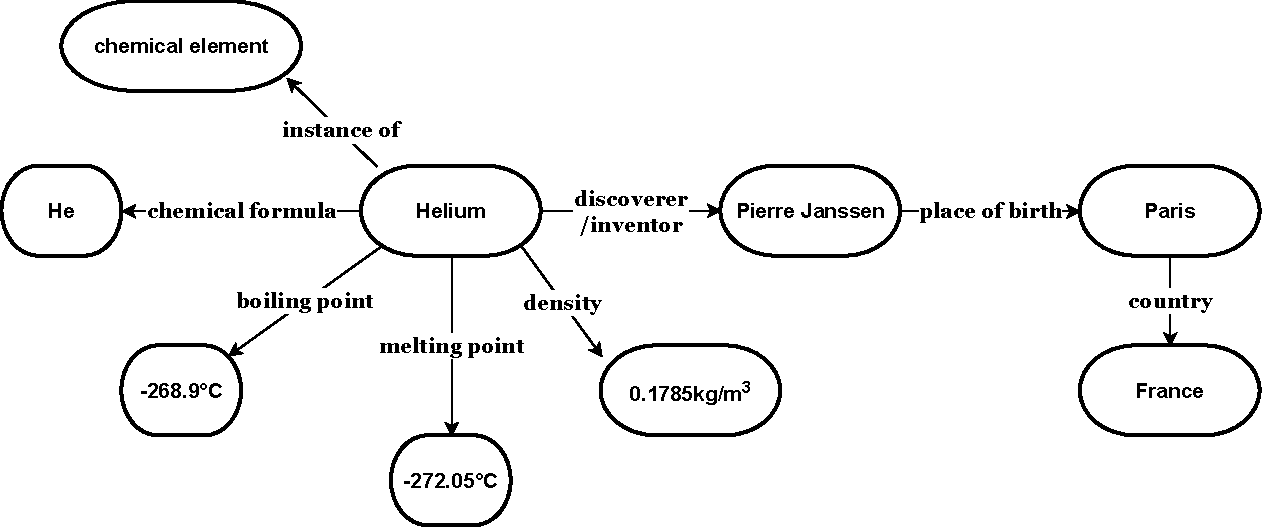
\includegraphics[width=0.80\linewidth]{images/del_graph.drawio.pdf}
  \caption{Directed edge-labelled graph describing Helium}
  \label{fig:figure 1}
\end{figure}

Resources in RDF are divided into groups known as classes. Ever member of a class is called an instance of that class. Properties describe the relationship between subject and object resources. In Figure~\ref{fig:figure 1} we see that Helium is an instance of the class chemical element. The property instance of describes the relation between the subject Helium and object chemical element.

In order to exchange graphs across the web we need to identify the resources uniquely. For this we use IRIs which are basically identifiers in RDF. The graph shown in Figure~\ref{fig:figure 1} can be represented using an RDF graph. Formally, the building blocks of RDF graphs are IRIs, literals and blank nodes. These are defined as follows.

\subsection*{IRI}
%\subsubsection{IRIs}
A Uniform Resource Identifier (\acrshort{URI}) is a sequence of a subset of ASCII characters that identifies any web resource by using a name, a location, or both. They have a scheme, authority, path, and query and fragment, where all parts other than scheme and path are optional. URIs are of the form \textbf{scheme:[//authority]path[?query][\#fragment]}. For example, \textit{http://www.wikidata.org/entity/Q560} is an IRI that identifies the chemical element Helium on Wikidata. A Uniform Resource Locator (\acrshort{URL}) is a subset of URI that is used to specify the location of a digital document.

An Internationalized Resource Identifier (\acrshort{IRI}) is a generalized form of URI that helps to distinguish resources with Unicode. Basically, the character set in URI is extended to the Universal Coded Character Set. This enables it to contain any Latin and non-Latin characters except the reserved characters.

In RDF an IRI is used as a name (can be thought of as an ID) for graph nodes. It defines the resources that appears as nodes or edge labels in a RDF graph. There are already several pre-existing IRIs available for common use. New domain specific IRIs can be created based on the application. However, we must ensure there no conflicts with other IRIs available on the web.

\subsection*{RDF Literals}
%\subsubsection{RDF Literals}

An RDF literal consists of three essential elements: a lexical value, a datatype IRI and an optional language tag. The lexical value is a string\footnote{RDF is based on Unicode strings} that corresponds to a particular literal value in the value space, where value space is the set of all possible values that a datatype can have. There are many datatypes\footnote{A full list is available on the W3C's section on RDF datatypes: www.w3.org/TR/2014/REC-rdf11-concepts-20140225/\#section-Datatypes} in RDF some of which are string, Boolean, decimal and integer.

The datatype IRI refers to a datatype that defines which strings are valid (belong in the lexical space), the value space and the lexical-to-value mapping \cite{ Bonduel2019}. This mapping is essentially a function that maps each string from the lexical space to an element in the value space. The \acrshort{W3C} standard XML Schema defines the datatypes and their IRIs. For example, decimals are identified by the IRI http://www.w3.org/2001/XMLSchema\#decimal. W3C has a good documentation on the different XML Schema built-in datatypes \cite{ R.Cyganiak2014}.

The optional language tag helps to provide human-readable labels to RDF literals. A literal is a language-tagged string is of the form "string"@language\footnote{Here language is a well-formed language tag (after \acrshort{BCP47})}. The datatype IRI\footnote{It is never used in syntax} of such literals is http://www.w3.org/1999/02/22-rdf-syntax-ns\#langString.

RDF literals are used to represent resources that have values belonging to datatypes. Each literal can have only one datatype. For example, the boiling point of Helium would be a RDF literal represented as \texttt{-268.9^^xsd:decimal} and its chemical formula as \texttt{"He"@en}, which is a language-tagged string. Literals are drawn as rectangular nodes in RDF graphs. 

\subsection*{Blank Nodes}
%\subsubsection{Blank Nodes}
A blank node in RDF, also known as a bnode, does not identify a specific resource as IRIs or literals do. It is used as a placeholder for some node, i.e., it is used to say that something with the given relationship exits at the position without specifying what the node is.


\subsection{RDF Graph}
\begin{definition}[RDF Graph]	
An RDF graph is a directed edge-labelled graph composed of a set of triples. These triples consist of the following elements:  

\begin{itemize}
	\item a subject (node) that is an IRI or a blank node; 
	\item a predicate (edge) that is an IRI; 
	\item an object (node) that is an IRI, a blank node, or a literal. 
\end{itemize}	
\end{definition}

Figure~\ref{fig:figure 2} shows an RDF graph based on our example represented in Figure~\ref{fig:figure 1}. Our main interest is in querying the knowledge graph Wikidata, and so all the data correspond to the resources in its knowledge base. In Wikidata the subject and object represent items, and the predicate represents properties. All items and properties are identified as Unique IDs. For example, the item \textit{Helium} has the ID of \texttt{Q560}, and the property \textit{chemical formula} has the ID \texttt{P274}. These are not understood by humans and have a label property that makes them understood. Moreover, items belong to the namespace \texttt{http://www.wikidata.org/entity/} (prefixed by \texttt{wd}) and properties to \texttt{http://www.wikidata.org/prop/direct/} (prefixed by \texttt{wdt}). As a result, \textit{Helium} would have the IRI \texttt{http://www.wikidata.org/entity/Q560} (\texttt{wd:Q560}) and \textit{chemical formula} the IRI \texttt{http://www.wikidata.org/prop/direct/P274} (\texttt{wdt:P274}). Section XYZ gives an elaborate understanding of entities and the namespaces they belong to in Wikidata.

From Figure~\ref{fig:figure 2} we understand that \textit{Helium} \texttt{(\gls{Q560})} is an \textit{instance of} \texttt{(P31)} of \textit{chemical element} \texttt{(Q11344)}. It has a human understandable english \textit{label} called \textit{helium} and the \textit{chemical formula} \texttt{(P274)} of \textit{He}. Its \textit{boiling point} \texttt{(P2102)}, \textit{melting point} \texttt{(P2102)} and \textit{density} \texttt{(P2054)} are \textit{-268.9~°C}, \textit{0.1785~°C} and \textit{-272-05~kg/m3} respectively. Helium has a \textit{discoverer/inventor} \texttt{(P61)} by the name of \textit{Pierre Janssen} \texttt{(Q298581)}. His \textit{place of birth} \texttt{(P19)} was \textit{Paris} \texttt{(Q90)} that belongs to the \textit{country} \texttt{(P17)} of \textit{France} \texttt{(Q142)}.

\begin{figure}[h]
  \centering
  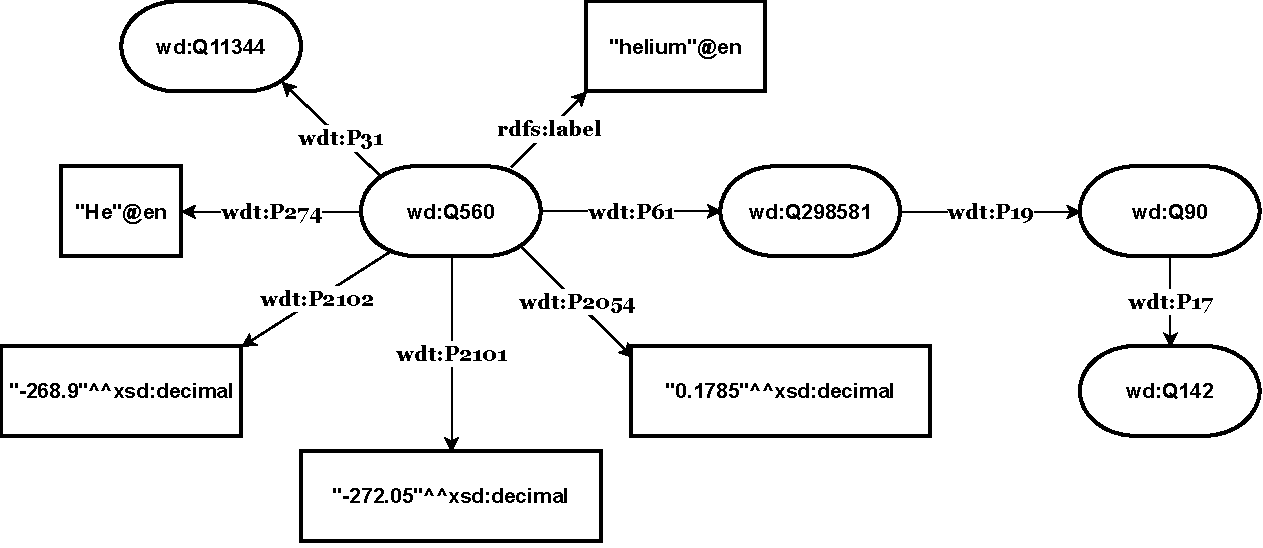
\includegraphics[width=0.75 \linewidth]{images/rdf_graph.drawio.pdf}
  \caption{RDF graph describing Helium}
  \label{fig:figure 2}
\end{figure}

%\begin{table}[b!]
%	\begin{center}
%		\caption{Abbreviation/IDs and their meanings.}
%		\label{tab: table 1}
%		\begin{tabular}{c|c}
%%			\textbf{Benchmarking tool} & \textbf{Resource monitoring tool} & \textbf{License} & \textbf{Updated} \\ \hline
%			wd & http://www.wikidata.org/entity/ \\ \hline
%			wdt & http://www.wikidata.org/prop/direct/ \\ \hline
%			rdfs & http://www.w3.org/2000/01/rdf-schema\# \\ \hline
%			Q560 & Helium \\ \hline
%			Q298581	& discoverer/inventor \\ \hline
%			Q90 & Paris \\ \hline
%			P31	& instance of \\ \hline
%			P274 & chemical formula \\ \hline
%			P2102 & boiling point \\ \hline
%			P2101 & melting point \\ \hline
%			P2054 & density \\ \hline
%			P61	& discoverer/inventor \\ \hline
%			P19	 & place of birth \\ \hline
%			P625 & coordinate location
%		\end{tabular}
%	\end{center}
%\end{table}


\subsection{Serialisations}
For exchanging graphs across the web, we need a syntactical representation of RDF. There are different formats available, the most common ones are N-Triples, Turtle, JSON-LD, RDF/XML and RDFa. In this report we focus on N-Triples and Turtle.

\subsubsection{N-Triples}
N-Triples represents RDF graphs in a simple line-based format\footnote{Full specification available at: https://www.w3.org/TR/n-triples/}. Every triple is encoded in a single line. The IRIs are written within pointy brackets and literals are written as lexical value\textasciicircum \textasciicircum datatype-IRI. Blank nodes are represented as \_:stringID, where stringID can be any string used to identify the blank node in the document. After every element of a triple there is a whitespace, and all the lines end with a dot. We can use comments using hash symbol after the end of every triple in a line or in a single dedicated line, and they are treated as white spaces. The files are saved with a \textit{.nt} extension.

Listing~\ref{listing:listing1} shows the representation of the RDF graph in Figure~\ref{fig:figure 2} in N-triples format. We have given line breaks for better readability.

\begin{minipage}{\linewidth}
\begin{lstlisting}[columns=fullflexible, label=listing:listing1, caption={RDF graph represented in N-triples syntax}]

<http://www.wikidata.org/entity/Q560> <http://www.wikidata.org/prop/direct/P31> 
%\phantom{<http://www.wikidata.org/entity/Q560> <http://www.}%<http://www.wikidata.org/entity/Q11344> .

<http://www.wikidata.org/entity/Q560> <http://www.w3.org/2000/01/rdf-schema#label> 
%\phantom{<http://www.wikidata.org/entity/Q560> <http://www.}%"helium"@en .

<http://www.wikidata.org/entity/Q560> <http://www.wikidata.org/prop/direct/P274> 
%\phantom{<http://www.wikidata.org/entity/Q560> <http://www.}%"He"@en .

<http://www.wikidata.org/entity/Q560>  <http://www.wikidata.org/prop/direct/P2102> 
%\phantom{<http://www.wikidata.org/entity/Q560> <http://www.}%"-268.9"^^<http://www.w3.org/2001/XMLSchema#decimal> .

<http://www.wikidata.org/entity/Q560> <http://www.wikidata.org/prop/direct/P2101> 
%\phantom{<http://www.wikidata.org/entity/Q560> <http://www.}%"0.1785"^^<http://www.w3.org/2001/XMLSchema#decimal> .

<http://www.wikidata.org/entity/Q560> <http://www.wikidata.org/prop/direct/P2054> 
%\phantom{<http://www.wikidata.org/entity/Q560> <http://www.}%"-272.05"^^<http://www.w3.org/2001/XMLSchema#decimal> .

<http://www.wikidata.org/entity/Q560> <http://www.wikidata.org/prop/direct/P61> 
%\phantom{<http://www.wikidata.org/entity/Q560> <http://www.}%<http://www.wikidata.org/entity/Q298581> .

<http://www.wikidata.org/entity/Q298581> <http://www.wikidata.org/prop/direct/P19> 
%\phantom{<http://www.wikidata.org/entity/Q560> <http://www.}%<http://www.wikidata.org/entity/Q90> .

<http://www.wikidata.org/entity/Q90> <http://www.wikidata.org/prop/direct/P17> 
%\phantom{<http://www.wikidata.org/entity/Q560> <http://www.}%<http://www.wikidata.org/entity/Q142> . 

\end{lstlisting}
\end{minipage}

\subsubsection{Turtle}
Turtle is an easy to read representation of RDF graphs. It extends the N-Triples format by providing several simplifications\footnote{Full specification available at: https://www.w3.org/TR/turtle/}. We can use prefix declarations and base namespaces at the beginning of the file to shorten IRIs. Turtle allows us to avoid repetition. We can use a semicolon at the end of a line instead of a dot if we know the next line has the same subject. Consequently, the next line will only have a predicate and object omitting the subject. Also, we can use a comma at the end of a line if we know the next line will start with the same subject and predicate. Analogously, the next line will only have a an object omitting the subject and the predicate. Blank nodes are represented using only square brackets. Additionally, we can provide predicate-object pairs within the square brackets to give further triples keeping the blank node as the subject. Turtle also provides a shorthand syntax for writing numbers. Numbers of the datatype integer, decimal and double can be written without quotes and datatype-IRIs. Boolean values can be written directly as either "\textit{true}" or "\textit{false}". The files are saved with a \textit{.ttl} extension.

Listing~\ref{listing:listing2} shows the representation of the RDF graph in Figure~\ref{fig:figure 2} in Turtle format. 

\begin{minipage}{\linewidth}
\begin{lstlisting}[label=listing:listing2, caption={RDF graph represented in Turtle syntax}]

PREFIX wd: <http://www.wikidata.org/entity/>
PREFIX wdt: <http://www.wikidata.org/prop/direct/>
PREFIX rdfs: <http://www.w3.org/2000/01/rdf-schema#>
PREFIX xsd: <http://www.w3.org/2001/XMLSchema#>
PREFIX geo: <http://www.opengis.net/ont/geosparql#>

wd:Q560 wdt:P31 wd:Q11344 ;
%\phantom{wd:Q560 }% rdfs:label "helium"@en ;
%\phantom{wd:Q560 }% wdt:P274 "He"@en ;
%\phantom{wd:Q560 }% wdt:P2102 -268.9 ;
%\phantom{wd:Q560 }% wdt:P2101 0.1785 ;
%\phantom{wd:Q560 }% wdt:P2054 -272.05 ;
%\phantom{wd:Q560 }% wdt:P61 wd:Q298581 .
wd:Q298581 wdt:P19 wd:Q90 .
wd:Q90 wdt:P17 wd:Q142 .

\end{lstlisting}
\end{minipage}


\section{Wikidata}
%\subsection{Wikidata}
Wikidata is a free and publicly available open knowledge base. It also acts as a central storage and data management platform for a variety of Wikimedia projects like Wikipedia, Wikitionary and Wikisource.  Wikidata was created in 2012 at Wikimedia Deutschland by a community of volunteers. These volunteers edit and control all content. As of December 2022, Wikidata has more 23000 active editors\footnote{https://wikidata.wikiscan.org/}. Wikidata provides a website where data can be viewed and also edited \cite{Foundationa}.

There is a wide range of applications for Wikidata. We previously mentioned that Wikidata functions as a database for Wikimedia community like Wikipedia. According to the lecture given by Krötzsch \cite{Kroetzsch2020}, it also has external uses in many large organizations like Eurowings, Google, Apple and Amazon for tasks such as data integration, authority control, identity providing and data-driven journalism. The lecture also mentions that in the field of research, Wikidata is used for collecting test data for knowledge graph related algorithms and training data for machine learning projects.

Wikidata is built on the RDF framework. However, it does not define its resources in terms of RDF. Instead, it has its own model known as Wikibase data model\footnote{https://www.mediawiki.org/wiki/Wikibase/DataModel}. This distinction creates an abstract layer between its model and RDF. Consequently, there are similarities with RDF’s W3C standards but there are also some important differences. For instance, the Wikidata property \textit{instance of} (\texttt{P31}) is semantically equivalent to the property \textit{rdf:type} in RDF. The value of \texttt{P31} is a class that is itself an item. Wikidata offers an explanation for some of the standards properties in Wikidata that correspond to the ones in RDF \cite{Foundation}. Statements (triples) in Wikidata can have annotations (qualifiers) and references.

The basic elements in Wikidata are entities, also known as resources. These are mainly items and properties. The next section describes entities in Wikidata. 

\subsection{Entities}
Wikidata maintains its data structure by pages. Each entity has a dedicated page for itself. Basically, every element on which Wikidata has structured data is known as an entity\cite{Erxleben2014}. Entities are identified by an unique ID and not by names or labels. Currently, Wikidata has mainly three types of entities – item, property and lexeme. Other extensions can define new entity types such as MediaInfo and subentities like Form and Sense. We will discuss about items and properties. The rest are out of the scope of this report.

Items are real-world objects, concepts or events. According to RDF terminology, items are instances and classes. Instead of a human understandable name, they are identified by a QID - an ID prefixed with the letter "Q" and followed a number. Items in Wikidata belong to the main namespace - \textit{http://www.wikidata.org/wiki/QID}. Every item constitutes of the following main parts - labels, descriptions, aliases, sitelinks and statements\cite{Erxleben2014}.

Labels, descriptions and aliases are multilingual which help to find the respective item. Since items are identified by an ID, these are used to identify the items clearly. Sitelinks provide links about an individual item in Wikidata to external pages on other Wikimedia sites such as Wikipedia and its other sister projects. The most important part are statements. 

A statement in Wikidata consists of a claim, references and a rank. Claims are property-value pairs, which along with the item form a RDF triple, where the item is the subject. Claims can also contain optional qualifiers that provide some additional information for the claim. This information is a property-value pair that refers to the main part of the statement instead of the item itself\cite{Erxleben2014}. References point to resources that support the claim. An item can have several statements for the same property, and all of them might not necessarily be important or relevant. Ranks are used as a quality factor to distinguish between several statements. A Wikidata statement can have one of three types of ranks - "normal", "preferred" and "deprecated". By default, a statement has the normal rank unless changed to preferred or deprecated. A statement with preferred rank means it should be given priority over the normal ranked statements. A deprecated rank indicates that the statement is incorrect or under discussion, and it may have a reference. Deprecated statements are kept either for the sake for completion or to prevent users from constantly adding or removing them. Wikidata has around 100 million items\footnote{https://grafana.wikimedia.org/d/000000167/wikidata-datamodel} and around 1.43 billion item statements as of December 2022\footnote{https://grafana.wikimedia.org/d/000000175/wikidata-datamodel-statements}.

Figure~\ref{fig:figure 3} shows an excerpt of the Wikidata page on the item Helium\footnote{https://www.wikidata.org/wiki/Q560}. We can see Helium has the QID of Q560, and has labels, descriptions and aliases in different languages. It has a sitelink for the item in Wikipedia offered in 186 languages. Helium has a statement that indicates that Helium has the instance of property with chemical element as the values. The property-value pairs follows, hydrogen and followed by, lithium are qualifiers. This statement hence gives us the information that Helium is an instance of chemical element, and it comes after the element hydrogen and if followed by the element lithium. This statement has no references and has the normal rank (indicated by the middle portion greyed).

\begin{figure}[h]
  \centering
  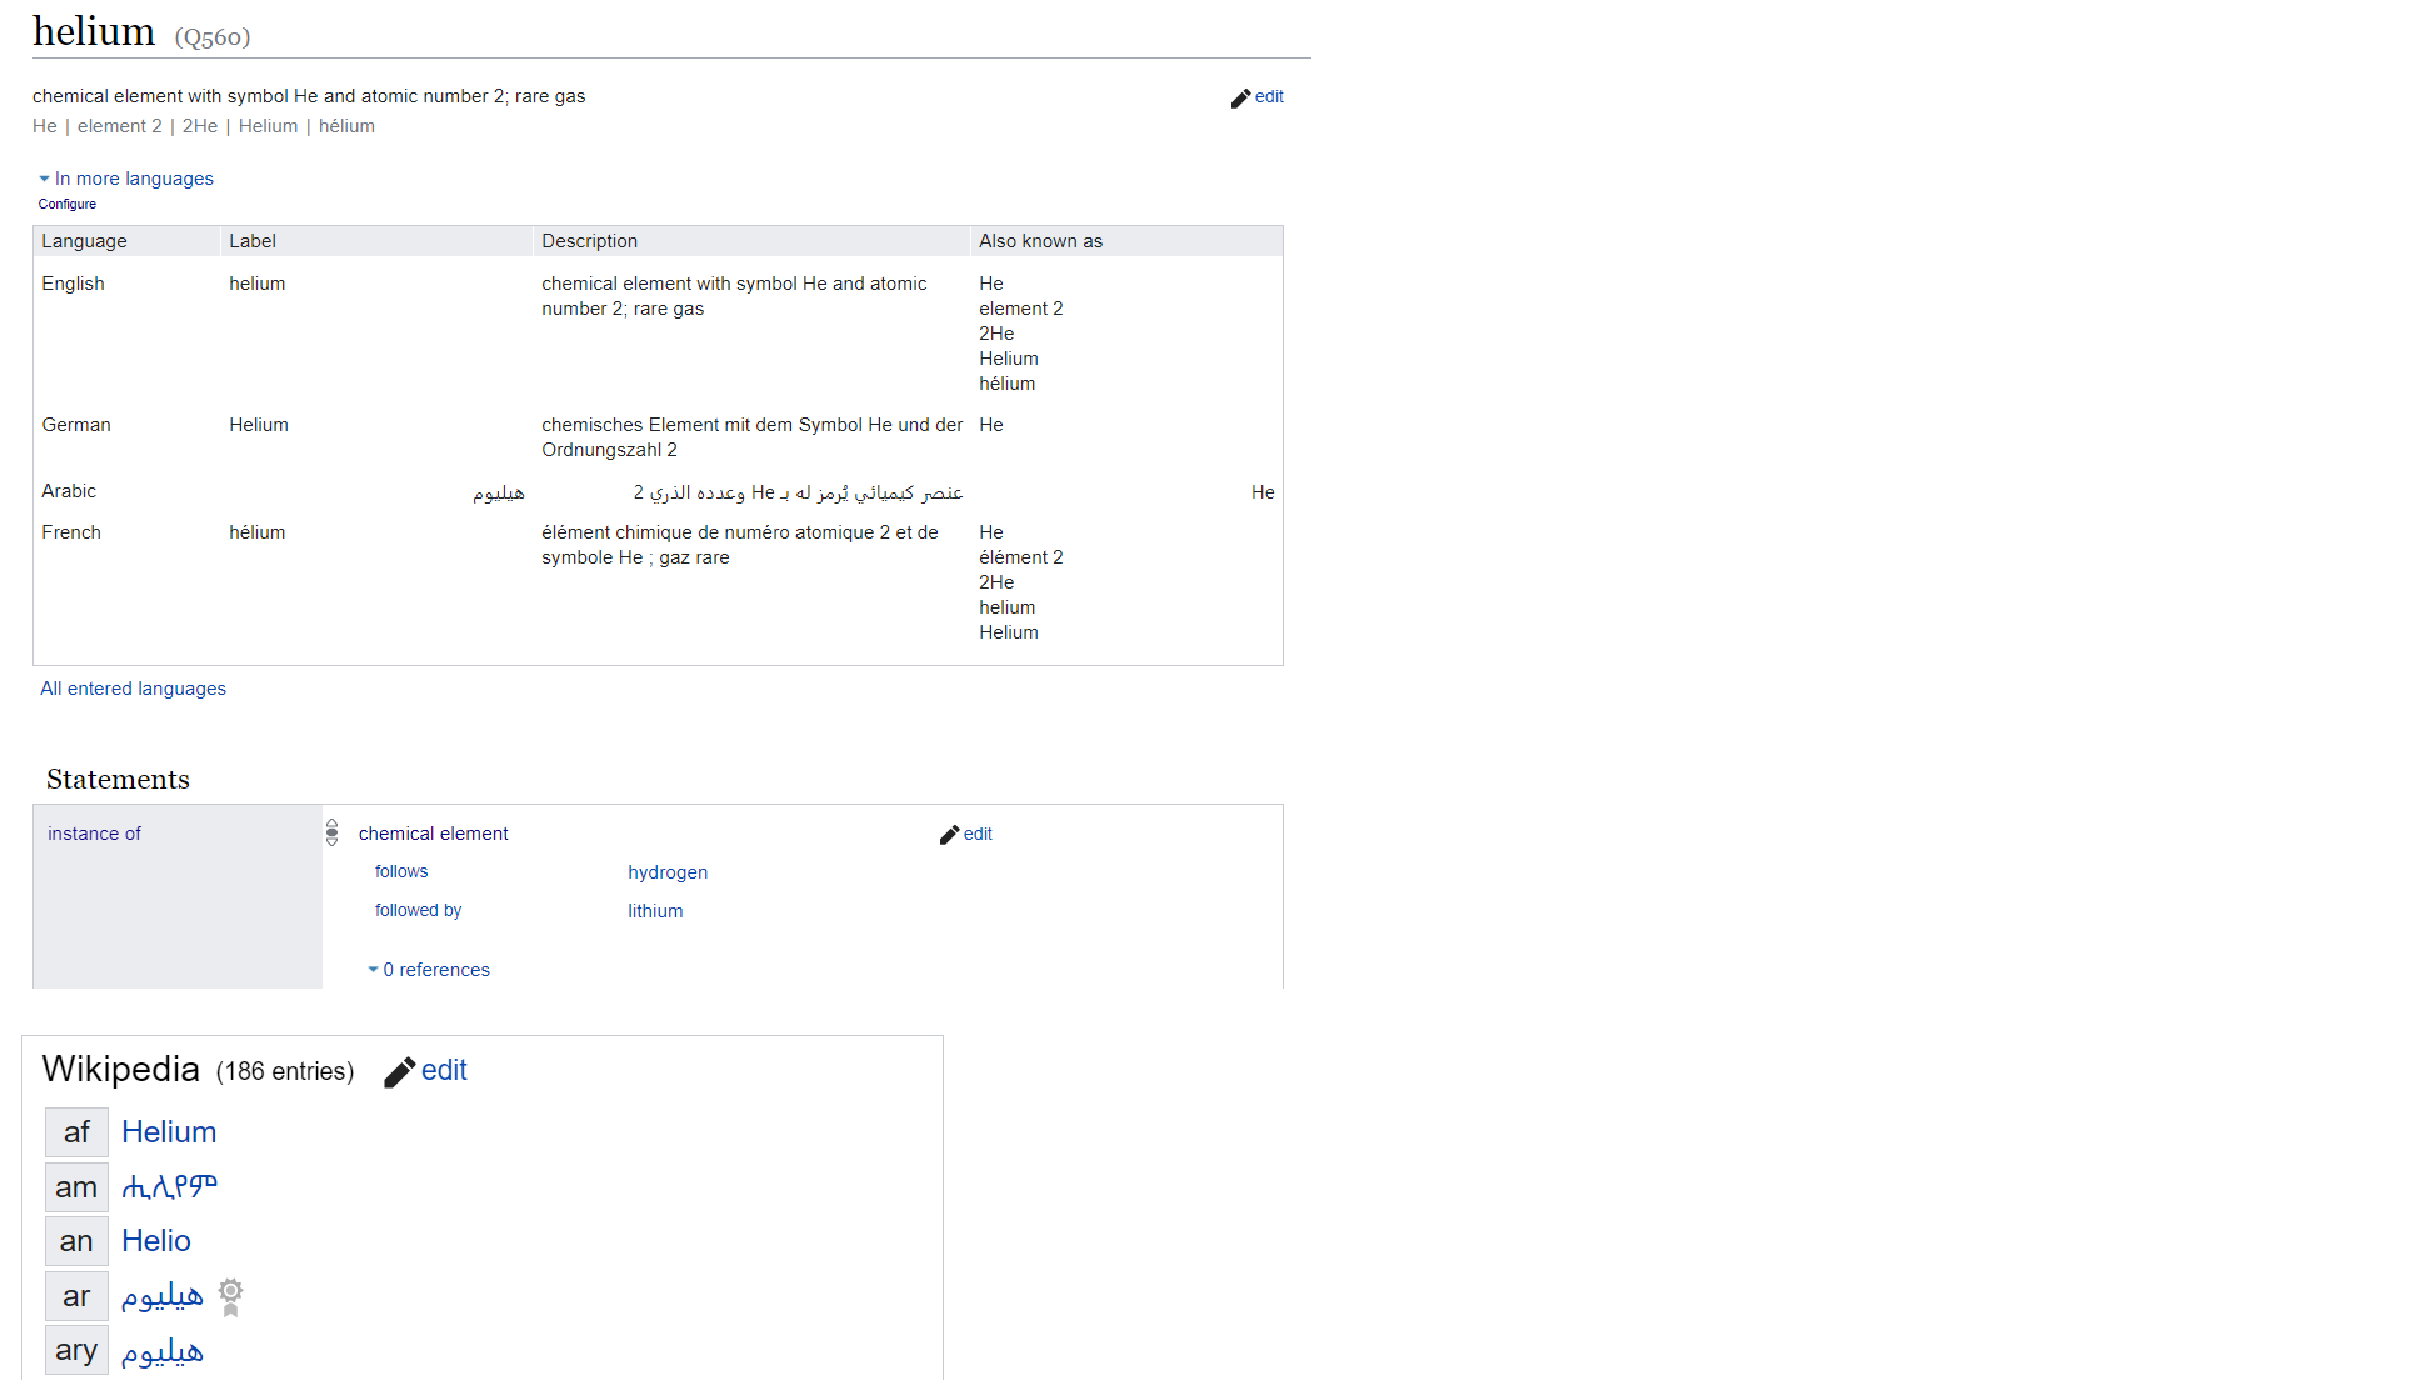
\includegraphics[width=0.75 \linewidth]{images/helium.pdf}
  \caption{An excerpt of the page on \textit{Helium} in Wikidata}
  \label{fig:figure 3}
\end{figure}

Properties in Wikidata resemble RDF properties and are essentially attributes for describing entities. They are identified by a PID - an ID prefixed with the letter "P" and followed a number. They belong to the property namespace in wikidata - http://www.wikidata.org/wiki/Property:PID. Like items, they also have labels, descriptions, aliases and statements but no sitelinks. However, they has an additional part called datatype that determines which values they accept, such as string, quantity and time\footnote{Wikidata provides a list of all the datatypes: https://www.wikidata.org/wiki/Special:ListDatatypes}.

Figure~\ref{fig:figure 4} shows an excerpt of the property instance of page on Wikidata\footnote{https://www.wikidata.org/wiki/P31}. The property has a PID of P31 along and with multilingual labels, descriptions and aliases. From the statement we understand that it this property also has an instance of property with Wikidata property being the value. The statement has no qualifiers or references, and has the normal rank. The instance of property accepts the datatype item as a value.

\begin{figure}[h]
  \centering
  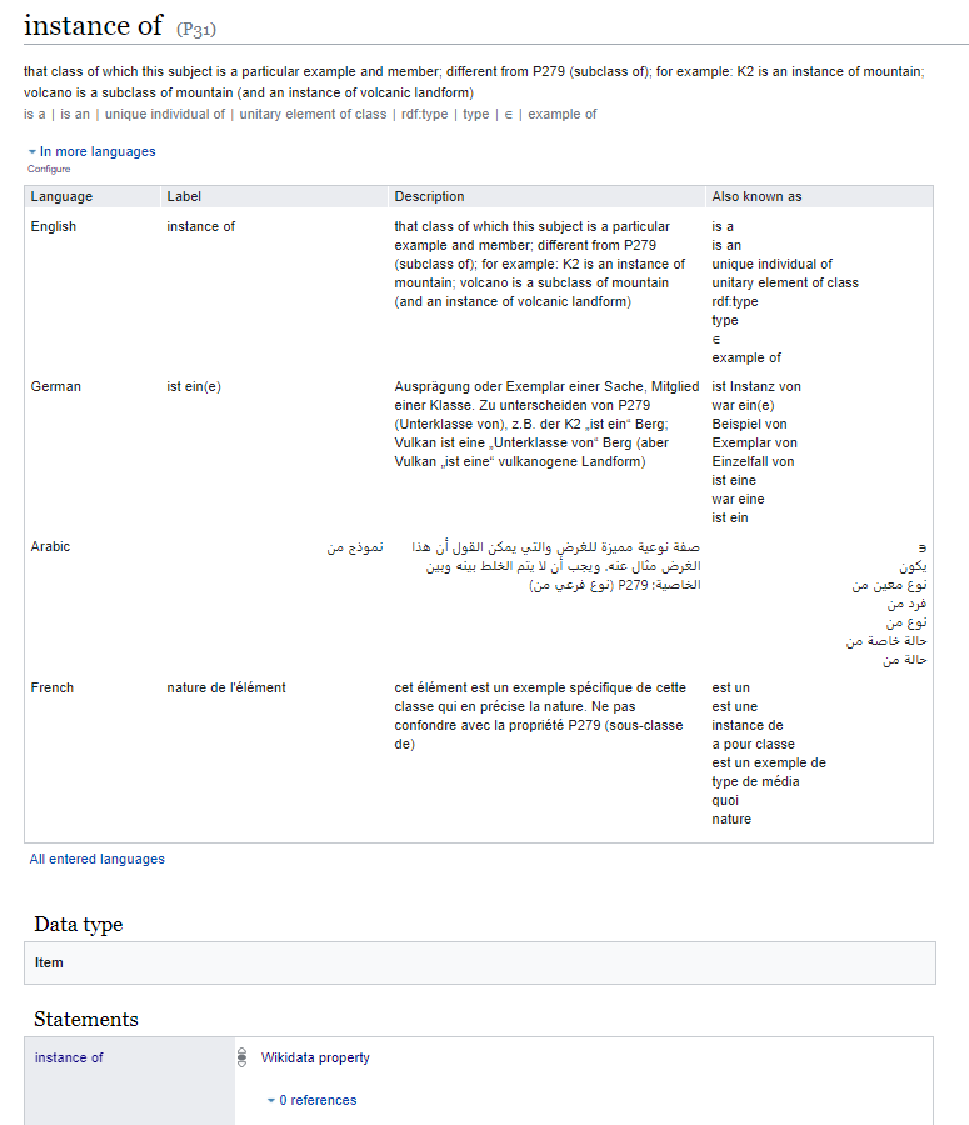
\includegraphics[width=0.75 \linewidth]{images/instance_of.pdf}
  \caption{An excerpt of the page on \textit{instance of} in Wikidata}
  \label{fig:figure 4}
\end{figure}

\subsection{Querying Wikidata}

The easiest and most popular way to query Wikidata is through the Wikidata Query Service (WDQS). This is Wikidata’s SPARQL endpoint. We can use this service two ways. Firstly, we can write queries in SPARQL directly on the web user interface of the service (footnote https://query.wikidata.org/) and obtain the results in different formats like table, tree, graph, etc. Secondly, the service can also be used pragmatically by submitting GET or POST requests\footnote{https://query.wikidata.org/sparql}.

Another popular way to query Wikidata is by using the Wikidata API\footnote{https://www.wikidata.org/wiki/Special:ApiSandbox}. However, this API should mainly be used when we want to edit the contents of Wikidata or get data about entities like revision history.

Wikidata dumps is useful when we know our result set will be significantly large or if we want to set up our own local query service. These dumps are full exports of all the available entities in Wikidata\footnote{https://dumps.wikimedia.org/}. To get started you should download the latest complete dump\footnote{https://dumps.wikimedia.org/wikidatawiki/latest/}. Wikidata also mentions some other ways to accessing Wikidata’s data like Search and Linked Data Fragments endpoint, the complete list and usage of which can be found on Wikidata’s Data Access webpage \cite{ Wikidata2022}.


\section{SPARQL}
%\subsection{SPARQL}
SPARQL Protocol and RDF Query Language (SPARQL) is a W3C recommended query language for RDF. This means it allows to query any data source that can be mapped to RDF. It is also a HTTP-based protocol for linked open data on the web. This enables the transmission of SPARQL queries and results between a client and a SPARQL engine. The first working draft for SPARQL was released in 2004 and it became a W3C Recommendation in 2008 \cite{Perez2009}. 

Queries in SPARQL are based on matching graph patterns and can be used to retrieve, add or delete data in the RDF based dataset. In section XYZ we saw that RDF data is based on triples - subject, object and predicate. Consequently, a query in SPARQL consists of a set of triple patterns. Each of the elements of the triple can be a variable (a string beginning with ? or \$) that needs to be queried. The solution to the variables is obtained by matching the query patterns to the triples in the dataset.

There are four forms of queries - SELECT, ASK, CONSTRUCT and DESCRIBE. 
\begin{itemize}
\item SELECT queries select some or all the pattern matches and provides the results in a tabular format
\item ASK queries check whether there is at least one match and the result is true or false
\item CONSTRUCT queries create an RDF graph based on the query results
\item DESCRIBE queries return a RDF graph providing additional information on each results
\end{itemize}

In our work, we only consider SELECT queries. These consist of the following major blocks:
\begin{itemize}
\item Prologue: PREFIX and BASE keywords that function similarly to those in RDF turtle format
\item Select clause: SELECT keyword followed by either a list of variables and variable assignments, or by *
\item Where clause: WHERE keyword followed by a query graph pattern to be matched
\item Solution set modifiers: Change the set of solutions using modifiers such as LIMIT and OFFSET
\end{itemize}

The select and where clauses are mandatory, the rest being optional. Other optional features are filters, groups, query operators such as UNION, OPTIONAL and BIND, and aggregates. A full specification for the query language can be found on the official W3C documentation\cite{Seaborn}.

Listing~\ref{listing:listing3} shows an example of querying Wikidata using SPARQL. We want to get a a list of all chemical elements, along with their English labels, that have a chemical formula, boiling point, melting point, density, an inventor/discoverer, birth place of that inventor/discoverer and the country that the place belongs to. Since there might be several results, we are limiting them to five using the LIMIT keyword. The namespace http://www.wikidata.org/entity/ is used for items when querying. We are interested in the truthy values of the properties and so the namespace http://www.wikidata.org/prop/direct/ is used for properties. Truthy values are essentially the values for which the statement has the best non-deprecated rank. This means that if a statement has preferred rank then that statement is considered to be truthy. Otherwise, the normal ranked statement is taken to be truthy. The PREFIX is optional since Wikidata recognizes the short forms wd and wdt automatically. Turtle syntax that we saw in section XYZ can be applied in SPARQL. The query can be run in Wikidata's query service\footnote{https://query.wikidata.org/}.  

\begin{minipage}{\linewidth}
\begin{lstlisting}[label=listing:listing3, caption={Querying Wikidata with SPARQL}]

PREFIX wd: <http://www.wikidata.org/entity/>
PREFIX wdt: <http://www.wikidata.org/prop/direct/>
SELECT *
WHERE {
  ?element wdt:P31 wd:Q11344 ;
  %\phantom{?element }% wdt:P274 ?element_formula ; 
  %\phantom{?element }% wdt:P2102 ?boiling_point ;
  %\phantom{?element }% wdt:P2101 ?melting_point ;
  %\phantom{?element }% wdt:P2054 ?density ;
  %\phantom{?element }% wdt:P61 ?discoverer .
  ?discoverer wdt:P19 ?place_birth .
  ?place_birth wdt:P17 ?country .
  FILTER(LANG(?element_label)="en")
}LIMIT 5

\end{lstlisting}
\end{minipage}

Table 1 shows the results obtained in a tabular form. Among the results, there is the element Helium (Q560) that we have used as an example in Fig 1 and Fig 2. 

\begin{table}[h]
	\begin{center}
		\caption{Results of the SPARQL query in Listing 2}
		\label{tab: table 1}
		\begin{tabular}{ccccccccc}
		
%		\textbf{element} & \textbf{element_formula} & \textbf{element_label} & \textbf{boiling_point} & \textbf{melting_point} & \textbf{density} & \textbf{discoverer} & \textbf{place_birth} & \textbf{country} \\ \hline
			\toprule
			
			\textbf{element} & \textbf{element\textunderscore formula} & \textbf{element\textunderscore label} & \textbf{boiling\textunderscore point} & \textbf{melting\textunderscore point} & \textbf{density} & \textbf{discoverer} & \textbf{place\textunderscore birth} & \textbf{country} \\ 
		
			\midrule
			
			wd:Q560 & He & helium	& -268.9 & -272.05 & 0.1785 & wd:Q298581 & wd:Q90 & wd:Q142 \\
			
			wd:Q560 & He & helium & -268.9 & -272.05 & 0.1785 & wd:Q950726 & wd:Q4093 & wd:Q145 \\ 
			
			wd:Q560 & He & helium & -268.9 & -272.05 & 0.1785	 & wd:Q127959 & wd:Q623765 & wd:Q145 \\ 
			
			wd:Q670 & Si & silicon & 4271 & 2570	& 2.329	& wd:Q151911 & wd:Q1451001 & wd:Q34 \\ 
			
			wd:Q568	& Li & lithium	& 1317	& 180.5	& 0.535	& wd:Q313568 & wd:Q10495519 & wd:Q34 \\
			
			\bottomrule

		\end{tabular}
	\end{center}
\end{table}

%\section{GraphQL}
%Stuff about GraphQL
%\subsection{GraphQL vs SPARQL}
%Stuff about GraphQL vs SPARQL
%
%
%\section{Literature Review}
%%\label{sec:literature}
%
%Stuff about GraphQL-LD and HypergraphQL and other tools do not have so many examples, and the ones that do are mainly for dbpedia.
%
%\section{GraphQL-LD}
%\subsection{JSON-LD}
%Elaborate on concrete JSON-LD represetation
%\subsection{Using Graphql-LD with Wikidata}
%
%\section{HypergraphQL}
%\subsection{Schema}
%Elaborate on schema of HypergraphQL
%\subsection{Using HypergraphQL with Wikidata}
%
%\section{GraphQL vs generated SPARQL queries}
%
%\section{Differences between the generated SPARQL queries by both tools}
%
%\section{Performance Evaluation}
%1. Evaluate performance of both approaches by writing SPARQL queries and equivalent GraphQL queries \\
%2. Discuss in how far the generated Sparql queries differ from the handwritten ones. \\
%3. analyze how well the approach scales with larger (deeper) GraphQL queries.
%
%
%
%
%
%\section{Effort for the setup}
%Evaluate/discuss the effort for the setup of both tools 
%
%\section{Default context}
%
%\section{Repository}
%
%
%\section{Challenges faced and Conclusion}
%\lipsum[1]

%\appendix
\singlespacing
\bibliographystyle{splncs04}
\bibliography{main}


\printglossaries
\end{document}
